
\documentclass[10pt,twocolumn,preprint]{elsarticle}
 \usepackage{lipsum}
 \usepackage{graphicx}
 \usepackage{natbib}
 \usepackage{url}
 \journal{Treatise in Geomorphology}
 

 \begin{document}

\twocolumn[{\begin{frontmatter}

     \title{A Community Approach to Modeling Earthscapes}

\author{Gregory E.\ Tucker}
\address{University of Colorado Boulder, Boulder, CO, USA}
\author{Rudy Slingerland}
\address{Penn State University, University Park, PA, USA}
\author{Jaia Syvitski}
\address{University of Colorado Boulder, Boulder, CO, USA}

     \begin{abstract} 
       Developing a unified, predictive science of surface processes requires a quantitative understanding of critical surface-dynamics processes. An efficient approach to acquire this understanding is community modeling, defined here as the collective efforts of individuals to code, debug, test, document, run, and apply a suite of modeling components coupled in a framework or community modeling system. The modeling components each consist of modular code, commonly with a standardized interface to allow different modules to communicate with other components written in a different programming language. The framework is a set of agreed-upon protocols that allow the components to function together. Because of the framework, users can assemble components coded and vetted by specialists into complex models tuned to their specific objectives. The advantages of community modeling are efficient use of community resources and more effective integration of scientists and software specialists.
     \end{abstract}


  \end{frontmatter}
}]
 
 \section{Background}
 
Starting in the 1970s, geoscientists began to translate conceptual models of complex, interacting geomorphic systems into computer codes to address problems that were not solvable analytically. The pioneering works of \citet{strelkoff1970numerical} solving the open-channel-flow equations, \citet{ahnert1976} modeling landform evolution, and \citet{harbaugh1970computer} modeling sedimentary systems showed us what was possible. With the advent of personal computers in the 1980s the trend accelerated, and journals such as \textit{Computers and Geosciences}, founded in 1976, were soon publishing over 100 computer codes a year. By the 1990s, the value of quantitative, model-driven science in Earth-surface studies was so apparent that funding panels began to expect it in proposals. A new generation of scientists more comfortable with algorithmic computation and, in some cases, better trained in mathematics led to a flowering in geomorphology. Noteworthy examples were insights gained in tectonic geomorphology from coupled tectonic and landscape evolution models \citep[e.g.,][]{beaumont1992erosional} and in the evolution of depositional systems from a new generation of sedimentary models \citep[e.g.,][]{slingerland1994simulating}.

During this exciting development phase, geomorphology codes were typically small, involving single developers. There were also very few repositories that would publish or make public your code. Some scientists distributed their code widely, but most code remained outside of the peer-review process.

\section{Concept of a Community Modeling System}
   
By 2002, it was apparent to many in the Earth-surface-science community that developing a unified, predictive science of surface processes was beset by two large and growing problems: the community was fragmented, and the quantitative understanding of critical surface-dynamics processes was uneven. To address these issues, the US National Science Foundation sponsored a workshop in 2002 directed toward developing a `Community Sediment Model.' It was envisioned as a suite of integrated, quantitative predictive models of basin and landscape evolution, encompassing both the subaerial and submarine realms. Subsequent workshops, guided by parallel developments in geophysics and climate science, refined the concept and, in 2007, led to the establishment and funding of the Community Surface Dynamics Modeling System (CSDMS). Other supportive community efforts included the Computational Infrastructure for Geodynamics (CIG) \citep{kellogg2018role}, the Chesapeake Community Modeling Program (CCMP), the Coastal Sediment Transport Modeling System \citep{warner2008development}, ROMS (the Regional Ocean Modeling System), and the Object Modeling System \citep{david2013software}. Community modeling as defined here involves the collective efforts of individuals to code, debug, test, document, run, and apply models and modeling frameworks \citep{voinov2010community}.

In its most basic form, a community modeling system is a suite of modeling components coupled in a framework \citep{voinov2010community}. The modeling components each consist of modular code, commonly with a standardized interface to allow different modules to communicate. The components performs specific tasks, such as reading digital elevation data from a file or computing grain-settling velocities according to a specific formula. Components typically can communicate with other components written in a different programming language and, thus, are different from ordinary subroutines, software modules, or classes in an object-oriented language. Individuals of relevant expertise freely give their time to code, debug, test, and document the various components and then donate them to the system. This by itself leads to an improvement in community efficiency. Community-developed components come together in a framework: a software library or system, designed around a set of standards and protocols, with which a user can run components, experiment with them by changing parameters in mid-run, and combine them to create integrated models. A framework allows one to assemble components coded and vetted by specialists into complex models tuned to their specific objectives. Community modeling brings several advantages. First, it makes efficient use of community resources by cutting redundancy among researchers and institutions. Second, community modeling promotes more effective integration of scientists and software specialists working on a particular Earth-surface system. Finally, it allows users, characteristically with valuable data sets, to participate in model definition and interaction with the data.



\section{Open-Source and Readily Available Code}

Community modeling relies on open-source code to address the practical need of contributing developers to examine and modify the code. Open-source code provides transparency, which is important because code is the ultimate statement of the scientific hypotheses embodied in a numerical model and its implementation. A scientific article may provide the theoretical equations, but the solution to these equations can take numerous forms, and each solution has its own pyramid of assumptions and limitations. Open-source code allows the possibility of full peer review and reproducibility of results---the foundation of modern science. Further, code availability should not depend on a gatekeeper, who subjectively determines who gets to see the code; this also runs contrary to the transparency needed in science.

Community modeling therefore relies on `software licensing and distribution designed to encourage use and improvement of software written by volunteers by ensuring that anyone can copy the source code and modify it freely' \citep{jesiek2003democratizing}. Open-source software is not necessarily freeware, but the source code must be freely available and modifiable. Its attributes include flexibility, tailorability, modularity, and open-endedness, in contrast to commercial software.

However, for scientific software to be fully transparent and support reproducible results, open source is not enough \citep{chen2019open}. Community modeling software should ideally support the FAIR principles: Findable, Accessible, Interoperable, and Reproducible \citep{wilkinson2016fair}. Findable means that the source code is included in a public, catalogued repository. Accessibility requires an open-source license along with adequate documentation, and software dependencies that are themselves accessible. Interoperability includes compatibility with at least one common operating system and, ideally, use of standardized interfaces and input/output protocols. Reproducibility, perhaps the biggest challenge \citep{barba2016hard}, requires that anyone can access and re-run the precise version of a code used to generate a result along with all required inputs \citep{fomel2009reproducible,peng2011reproducible,stodden2013setting}.

\section{Community Modeling and the CSDMS Approach}

The largest and most inclusive communal modeling effort in hydrology, geomorphology, sedimentology, and stratigraphy, with overlap in related fields of environmental engineering, oceanography, and tectonics, is the Community Surface Dynamics Modeling System or CSDMS (pronounced `systems') \citep{tucker2021numerical}. CSDMS is an integrated community of experts developing and disseminating integrated software modules that predict the movement of fluids (wind, water, and ice), sediment, and solutes in landscapes, seascapes, and their sedimentary basins. The organization operates under a grant from the US National Science Foundation (NSF). CSDMS Working Groups self-organized from the scientific community identify important knowledge gaps and encourage code development in those areas. The CSDMS approach to community modeling uses three complementary technologies: an online catalog and repository to support sharing model codes; a framework for creating, running, and coupling models as interoperable modules; and a component-based programming library for building a new generation of models.

The CSDMS Model Repository comprises a searchable inventory of models, some of which have been made into interoperable components that users can link through the CSDMS model-coupling framework. The Model Repository serves as the geomorphology community's platform for open-source code sharing, which is often required by funding agencies and (increasingly) journals. As of April 2021, the CSDMS model repository included nearly 400 community-built codes, ranging from single subroutines to large, integrated numerical models. Of these, about two dozen offer a standardized interface and a Python-language front end that allows them to operate as components in an integrated framework. Each entry in the Repository includes extensive metadata about the code, including information about processes, technical specifications, inputs/outputs, and a bibliography. For each code, the citations to references that describe or apply it are used to provide an h-index for that particular code, which provides prospective users an indication of how widely the program is used. The source codes themselves are either hosted on a separate website by the developers, or by the CSDMS Integration Facility in a GitHub repository; in either case, the Repository includes links directly to the source code.

To create a modeling environment in which individual pre-existing model codes act as standardized, interoperable components, several resources are needed. The first is an interface standard, or application programming interface (API), which comprises a list of public functions that a code provides. The standard specifies the function names, call signatures, return types, and intended functionality. A code that provides all of the specified functions can be said to meet that particular interface standard. Providing a standardized set of functions is one step toward making a code operable by an external script or other program. To meet the needs of a modular modeling framework, CSDMS develops and supports an interface standard known as the Basic Model Interface (BMI), which provides functions to handle operations that are common to most gridded numerical models, including initialization, advancing iteratively in time, querying state variables and parameters, and changing values. Version 2.0 of the BMI specification is described by \citet{hutton2020basic}, and discussed with examples by \citet{tucker2021numerical}. The advantage of an interface standard like BMI is that all codes that adopt it express the same basic control functionality, which greatly simplifies the task of operating them as modules and exchanging data between modules. The BMI has been used in a variety of coupled-modeling applications, such as flood hydrology \citep{hoch2019advancing,hoch2019evaluating}, rainfall-runoff \citep{piper2020coupling}, river management \citep{den2020virtual}, delta evolution \citep{ratliff2018exploring,ratliff2021modeling}, and permafrost \citep{wang2020sensitivity}. A related protocol is a set of standard names for data items, based on a general blueprint for variable naming called the Scientific Variables Ontology \citep{stoica2018ontology,stoica2019incorporating,stoica2019scientific,stoica2020github}, which further simplifies the process of data exchange.

A second requirement for a modular environment is language standardization. Model programs in geomorphology and related sciences are written in a variety of languages, including Fortran, C, C++, and Python, to name a few. The CSDMS approach uses Python as a hub language. Python is  popular in the science community as a high-level interpreted language that allows for rapid prototyping, and it features a rich set of third-party open-source libraries for numerical computing, data analysis, and plotting. Once a code is equipped with a BMI in its native language, a software tool called babelizer is used to compile the code as a binary library that can be imported into Python. A user can then operate that model, using Python implementations of BMI functions, in a Python script, shell, or Jupyter notebook.

The third requirement is a model execution and coupling framework. In its early research, the CSDMS Integration Facility experimented with graphically based frameworks. One discovery was that many problems of interest to the geomorphology community require a level of finesse and customization that can only be achieved with a programmatic, script-based framework.  For this reason, the current CSDMS approach provides a script-based framework that takes advantage of the power and popularity of the scientific Python. A code that has been equipped with a BMI and then compiled as a Python-readable binary library is said to have been `wrapped' as an interoperable component. Because any such component can be imported and run in a Python script, Python itself becomes the model coupling and execution framework. One can, for example, write a script in which two components are initialized, and then run in a loop in which the components iteratively exchange data (Figure~\ref{fig:pymt-cem-waves-example}). Alternatively, components that represent different terms in a governing equation could be queried for their derivatives, and those derivates then used to compose a matrix equation that is solved using Python matrix inversion utilities. These inherent framework capabilities are further enhanced with a Python package called the Python Modeling Tool (pymt), which provides several additional elements of functionality for coupling models. These include, for example, a standard-syntax setup function that creates the necessary input files for each component, and grid-mapping utilities that use interpolation to translate quantities from one grid to another (Figures~\ref{fig:pymt-cem-waves-example}, \ref{fig:child-sedflux}). The Python Modeling Tool makes it possible not just to assemble coupled, component-based models, but also to operate these models in a real-time experimental mode: advancing for a period of time, pausing to plot and analyze, modifying parameters, and continuing. In addition to its obvious educational application, this ability to play around with models provides a great way to generate new ideas and insights.

\begin{figure*}[htbp]
   \centering
   \includegraphics[width=\textwidth]{figures/pymt_cem+waves_example.pdf} % requires the graphicx package
   \caption{Simple example of model coupling using a Python script and the Python Modeling Tool (pymt). This example uses two models: the Coastline Evolution Model (CEM) and Waves, both written in C. The BMI functions \texttt{initialize()}, \texttt{update()}, \texttt{get\_value()}, and \texttt{get\_value()} are used to control the two codes; the pymt function \texttt{setup()} is used to create the necessary input files for each one. The complete example can be found in the CSDMS pymt tutorials collection.}
   \label{fig:pymt-cem-waves-example}
\end{figure*}

\begin{figure}[htbp]
   \centering
   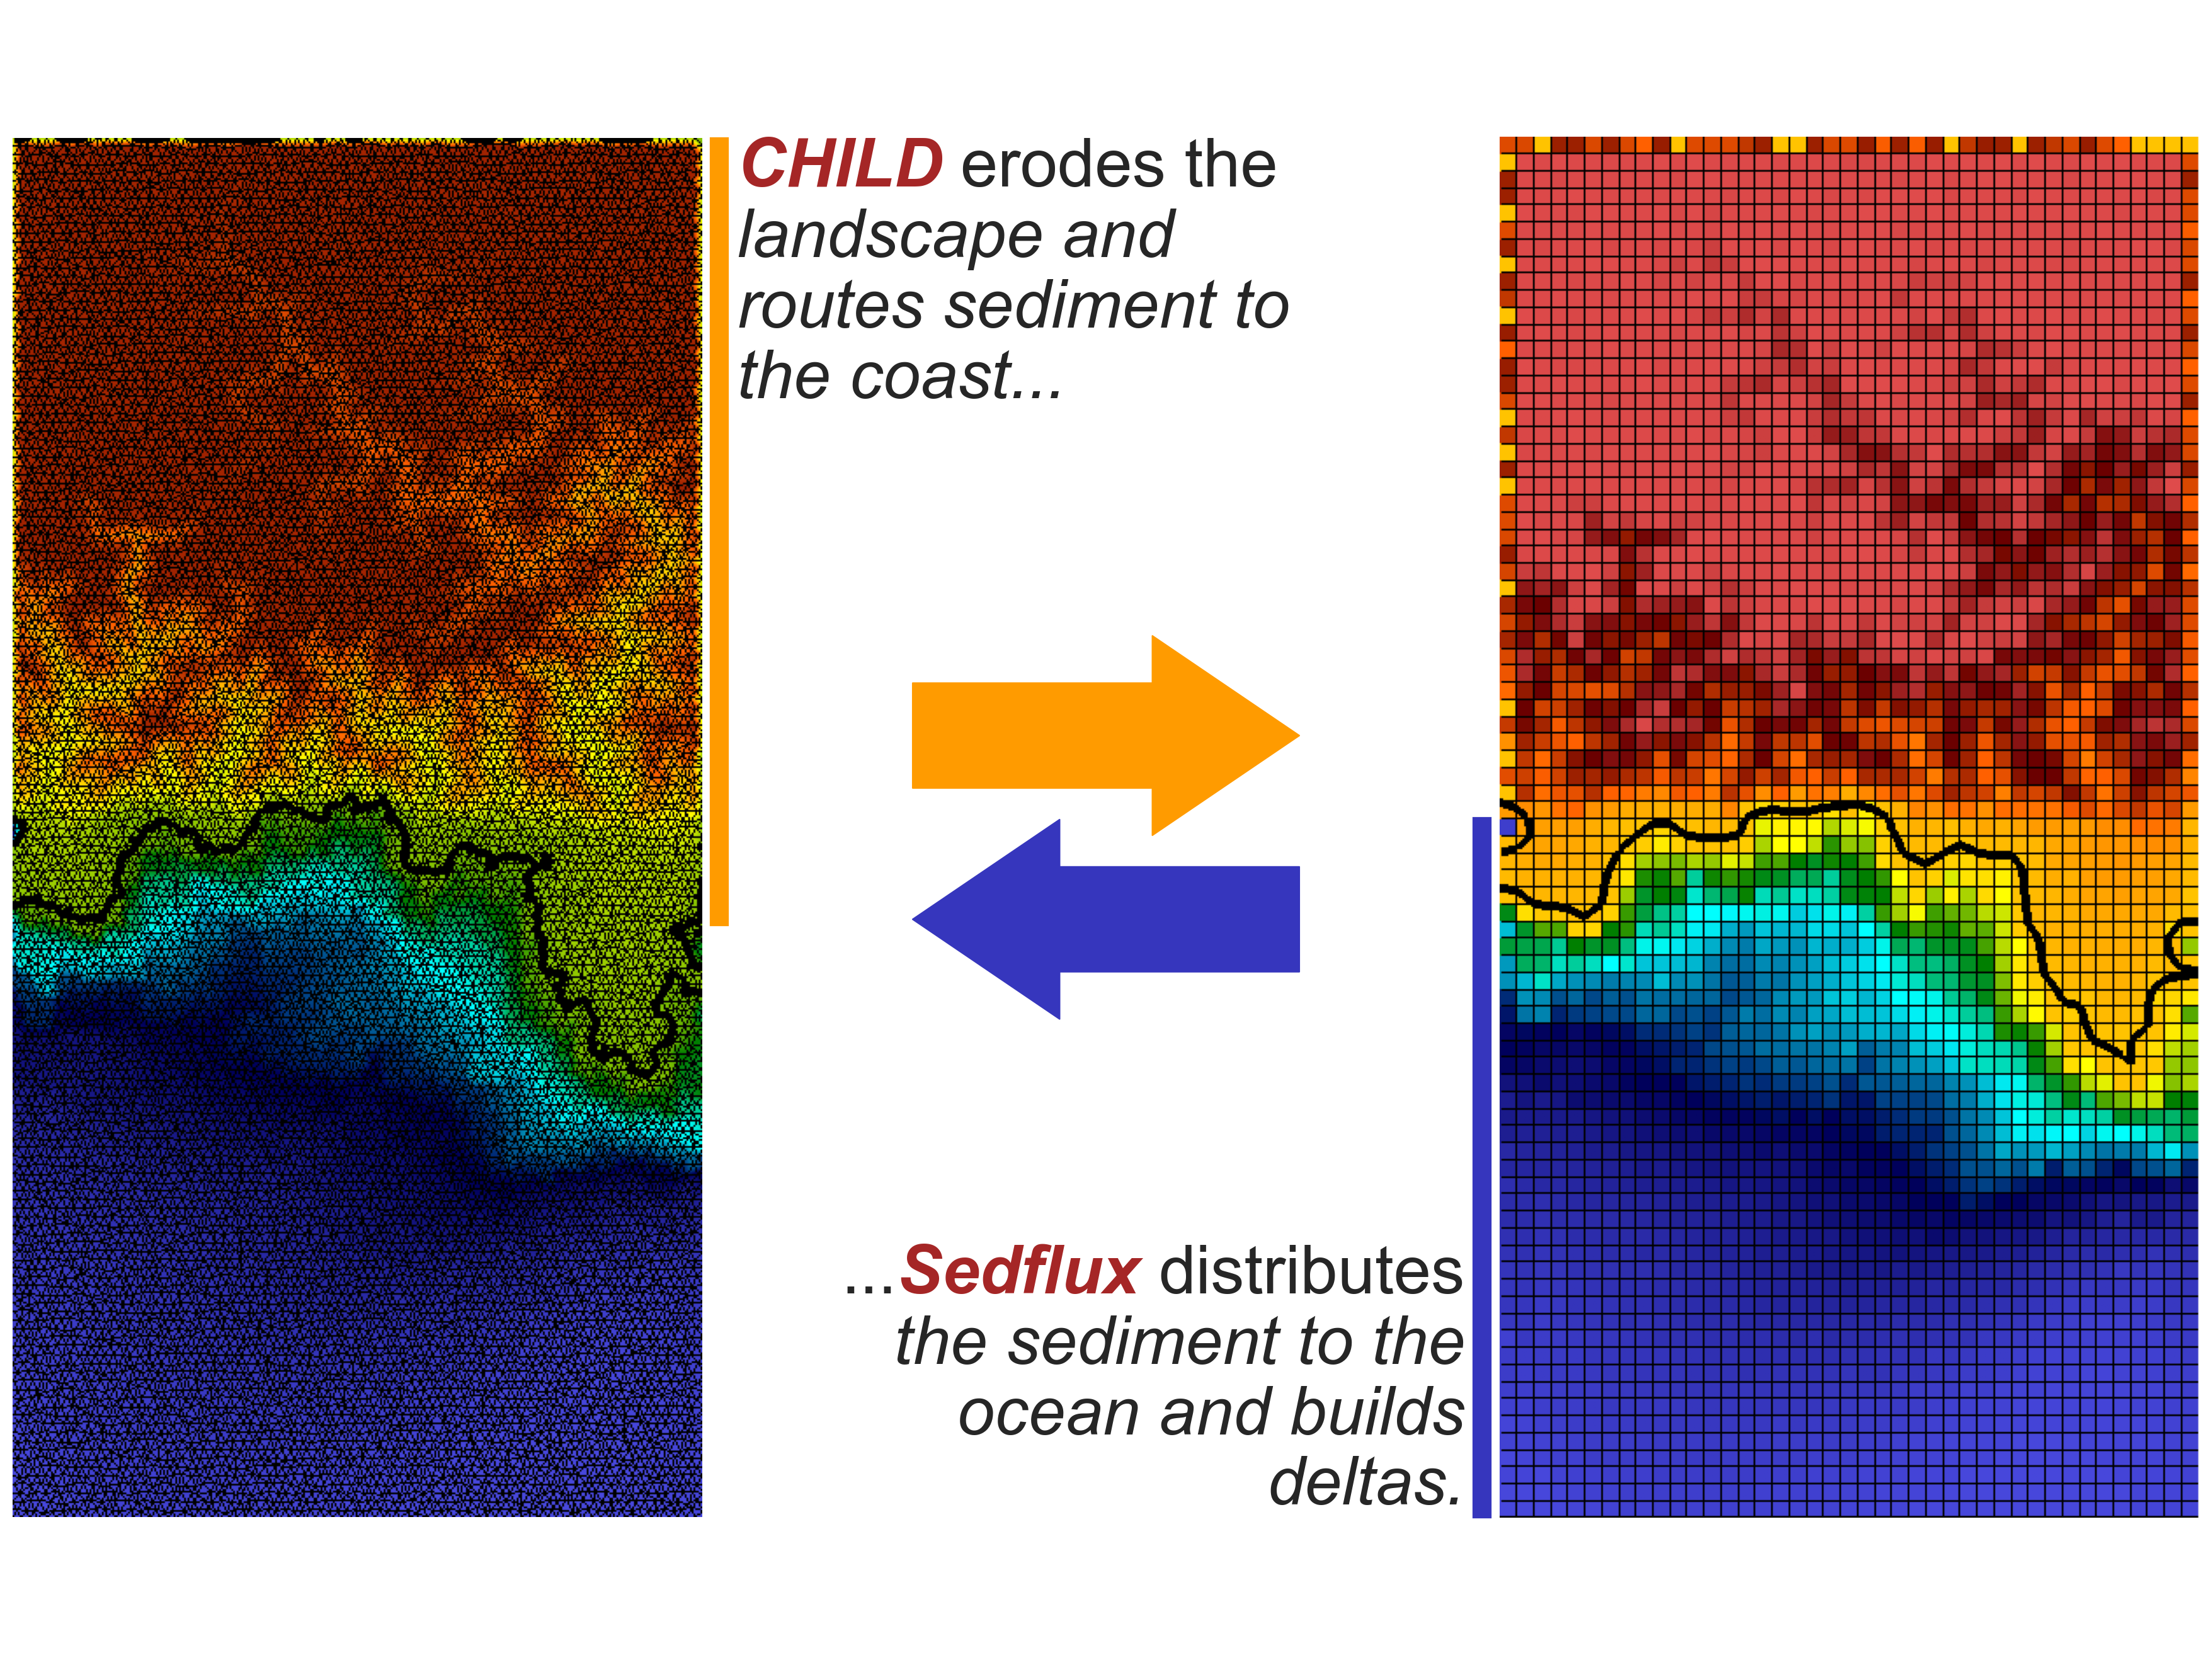
\includegraphics[width=\columnwidth]{figures/child_sedflux.png} 
   \caption{Output from a pymt integrated model that couples two components with different grid types. The CHILD model \citep{tucker2001channel}, written in C++, computes subaerial erosion, sediment transport, and landscape evolution on a triangulated irregular network of grid nodes. The Sedflux3d model \citep{hutton2008sedflux}, written in C, computes submarine transport, deposition, and stratigraphy on a regular grid. Pymt grid-mapping functions are used to interpolate between the two grid types. Coupling these two models as pymt components results in an integrated source-to-sink modeling framework. (Black line indicates shoreline; dark blue colors are deep water, and dark red colors are high elevations.)}
   \label{fig:child-sedflux}
\end{figure}

New discoveries and new data in geomorphology motivate new models. To accelerate the development and exploration of a new generation of models, CSDMS deploys Landlab Toolkit: a Python-language programming library that supports modular model-building \citep{hobley2017creative,barnhart2020short}. Landlab complements the BMI-pymt framework while overcoming some of its limitations. One of those limitations is memory usage: because each BMI-pymt component manages its own data, there is inevitable duplication among components that represent the same state variables. Another limitation arises from the need to support multiple languages: the interface must be relatively simple, and cannot take advantage of advanced design features, such as built-in array types, that only a subset of languages support. Landlab takes advantage of the high-level language features of Python, such as object-oriented capabilities, to enable modular model construction at a more granular level. One of its key features lies in grid support. A Landlab grid is a self-contained data object. A programmer can create a grid object of a given type and geometry in a single line of Python code. Grids are represented as graphs (in the sense of graph theory), with each grid comprising a set of primitive geometric elements such as nodes, links, and cells. As a result, the same data structures can be used to represent grids of different types, such as raster, hex/trigonal, or unstructured. This provides the novel ability to operate the same numerical model with different grid types. State variables in a model are handled by adding arrays of data (`fields') to elements of the grid; for example, a heat-flow model might assign an array of temperature values to grid nodes, and an array of heat-flux values to links. 

The Landlab Toolkit provides utilities to handle common operations in a numerical model, such as numerical functions (e.g., gradient, divergence), input of parameter values from a standard-format text file, and output of data in standard file formats such as NetCDF. The real power of Landlab, however, comes in its use of modular components. A Landlab component is a code implemented as a Python class that implements a numerical solution for a particular process or analysis function. For example, a Landlab component might implement a finite-volume solution to the conductive heat-diffusion equation. Landlab components use a lightweight interface that includes a constructor (initialization) function and an action function that advances the component in time (if it is a time-advancing process) or otherwise performs its calculation. A programmer can build an integrated model by importing a set of components, initializing them, and operating them in a time loop. The components share the same grid and associated fields of data, thereby avoiding duplicated memory usage.

Figure~\ref{fig:islandexample} shows an example of a Landlab-built source-to-sink model that simulates the evolution of a large oceanic island undergoing active asymmetric rifting. The model is implemented as a Python script that integrates Landlab components for rift tectonics, flexural isostasy, flow routing on land, fluvial erosion and sedimentation, and marine sediment transport. 

Landlab has been used in a wide variety of research applications, many of which span boundaries between traditional disciplines and domains. Some examples include post-glacial landscape evolution \citep{lai2018modeled,barnhart2020inverting1,barnhart2020inverting2}, tectonic geomorphology \citep{gray2017off,reitman2019offset,zebari2019relative,lai2020tectonic,tucker2020modeling,pan2021numerical,shen2021modeling}, lateral stream erosion \citep{langston2018developing}, lithologic effects \citep{glade2019canyon,sheehan2020migrating}, gully erosion \citep{walker2020multi}, fluvial sediment routing \citep{pfeiffer2020networksedimenttransporter}, hillslope morphology \citep{tucker2018lattice}, landsliding \citep{strauch2018hydroclimatological}, erosion forecasting \citep{barnhart2020projections}, glacial erosion \citep{lai2020tectonic}, vegetation and slope-aspect controls on erosion \citep{pelletier2017way,schmid2018effect,carriere2020impact}, river sediment provenance and geochemistry \citep{sharman2019conversion,lipp2020river}, surface-water hydrology \citep{adams2017landlab,anand2020linear}, groundwater \citep{litwin2020groundwaterdupuitpercolator}, stream capture impacts on biological evolution \citep{lyons2020topographic,lyons2020speciesevolver}, terrestrial ecology \citep{evans2020beyond}, and STEM education \citep{bandaragoda2019enabling}. Because anyone can contribute a new component or utility, Landlab functions as a resource by and for the scientific community.

\begin{figure*}[htbp]
   \centering
   \includegraphics[width=\textwidth]{figures/island_example210322.pdf} 
   \caption{Example source-to-sink simulation of an island microcontinent undergoing oblique tectonic extension and stochastic variation in sea level. Domain width is 250~km. (a) Topography and drainage patterns after 1.05~my of active rifting. Lagoons on east side reflect combined eustatic and flexural isostatic drowning of portions of the coastal plain. (b) Thickness of sedimentary deposits (blue colors) and exhumation depth (red colors). Code was written in Python using the Landlab Toolkit, and combines several Landlab components to create an integrated source-to-sink model: tectonic extension (\textit{ListricKinematicExtender}), flexural isostasy (\textit{Flexure}), flow routing across terrain (\textit{FlowAccumulator, FlowDirector, LakeMapperBarnes}), fluvial processes (\textit{ErosionDeposition}), and submarine sediment transport (\textit{SimpleSubmarineDiffuser}).}
   \label{fig:islandexample}
\end{figure*}







\section{Challenges and Opportunities}

Community modeling software does not simply evolve on its own, but instead requires intentional effort. Thus, to gain the benefits of community modeling, some level of investment in coordination and oversight is needed. A related challenge lies in recognizing and thereby incentivizing individual contributions. Well-documented, peer-reviewed code should be seen as worthy of merit, with effective venues for peer review, publication, and citation. New developments in peer review of codes, such as provided by research software journals like the \textit{Journal of Open Source Software}, can help by giving formal academic credit for software development. Because it is the code itself that undergoes evaluation, as opposed to a paper describing it, direct software peer review can improve the quality, reliability, and reusability of community modeling codes. But these contributions must be recognized and rewarded by universities, research agencies, and other institutions. Another challenge lies in community training. Geomorphologists are often self-taught programmers, and may be unaware of tools and practices that can greatly improve the quality of their code contributions. Organizations like CSDMS are working to fill this gap with educational resources and programs, but there remains a role for universities and funding agencies as well.


\section{Summary}

Community modeling efforts, such as CSDMS, provide a competitive yet cooperative environment that can produce more reliable and more flexible simulation models than individuals working alone. Freely available open-source code with a standardized interface eliminates the endless rewriting of the same initial algorithms, allowing more time spent on new advances. The CSDMS protocols create honesty in what modelers claim, and the CSDMS architecture allows for faster verification and comparison of different approaches on new data sets. Communication is greatly increased among users and coders, and, therefore, a more integrated community is built. If a new and improved model component is developed, then this new component is provided with faster penetration into the community and likely will replace older components. New model couplings will allow hypothesis testing, sensitivity experiments on key parameters, and the identification of new avenues of research.


\bibliographystyle{agu08}
\bibliography{gt_library.bib}

\end{document}
